\begin{pastexam}[label={px:ntut-115-ci-03}]{北科大資工所 115 學年度 第 3 題}
（計算）

Let $|T|$ denote the number of nodes of a binary tree $T$. If $|T|$=0 or $|T|$=1, there is only one
binary tree. If $|T|$=2, then there are two distinct binary trees. (10\%)
\begin{enumerate}[label=(\arabic*)]
\item When $|T|$=3, how many distinct binary trees are there? (3\%)
\item We are now interested in deriving the total number of distinct binary trees when $|T|$=
$n$. Suppose $D_n$ denote this number. Please write a recurrence equation to obtain $D_n$. (3\%)
\end{enumerate}
Recall the optimal binary search tree problem and one can get an optimal binary search tree with
given access frequencies of keys among different possible binary search trees. Suppose that we are
given four keys, $a_1$, $a_2$, $a_3$, and $a_4$, with the following access frequencies ($p_i$) as
well as the unsuccessful access frequencies ($q_i$) to the gaps ($e_i$), where
$e_i$=($a_i$, $a_{i+1}$), $i$ = 1, 2, and 3; $e_0$=($-\infty$, $a_1$); and $e_4$=($a_4$, $\infty$).
Please answer the following two questions (3) and (4).
\begin{center}
\begin{tabular}{r|c|c|c|c|c}
$i$ & 0 & 1 & 2 & 3 & 4\\\hline
$p_i$ (for $a_i$) & -- & 3 & 3 & 1 & 1\\\hline
$q_i$ (for $e_i$) & 2 & 3 & 1 & 1 & 1
\end{tabular}
\end{center}
\begin{enumerate}[label=(\arabic*),start=3]
\item Which key will be located at the root of the resulting optimal binary search? (2\%)
\item Which key will be located at the parent of the node storing key $a_4$? (2\%)
\end{enumerate}
\end{pastexam}

\begin{pastsoln}
答案：(1) $5$；(2) $D_0 = 1$，$D_n = \sum_{i=0}^{n-1} D_i D_{n-1-i}$（$n \ge 1$）；(3) $a_2$；(4) $a_3$
（有另一棵一樣好的樹，見下面的說明）。

(1)(2) 是資結書第~7~章（二元樹計數），(3)(4) 是第~18~章（最佳二元搜尋樹）；配分 (1)(2) 比較重，
放在第~7~章。 (3) 原題的「optimal binary search」少了「tree」。

\textbf{(1)} 三個節點：根固定，剩下兩個節點分給左右子樹，可以是 $(2, 0)$、$(1, 1)$、$(0, 2)$。 兩個節點的
子樹有 $2$ 種，所以共 $2 \cdot 1 + 1 \cdot 1 + 1 \cdot 2 = 5$ 種：
\begin{center}
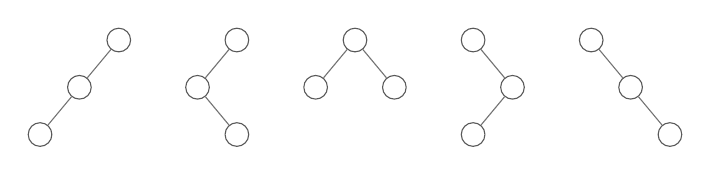
\begin{tikzpicture}[x=0.5cm,y=0.6cm,
  tn/.style={circle, draw=black!65, minimum size=0.3cm, inner sep=0pt}, te/.style={draw=black!55}]
\foreach \x/\a/\b in {0/-1/-2, 3/-1/0, 6/0/0, 9/1/0, 12/1/2}{
  \node[tn] (r\x) at (\x,0) {};
}
\node[tn] (a1) at (-1,-1) {}; \node[tn] (b1) at (-2,-2) {}; \draw[te] (r0)--(a1)--(b1);
\node[tn] (a2) at (2,-1) {};  \node[tn] (b2) at (3,-2) {};  \draw[te] (r3)--(a2)--(b2);
\node[tn] (a3) at (5,-1) {};  \node[tn] (b3) at (7,-1) {};  \draw[te] (a3)--(r6)--(b3);
\node[tn] (a4) at (10,-1) {}; \node[tn] (b4) at (9,-2) {};  \draw[te] (r9)--(a4)--(b4);
\node[tn] (a5) at (13,-1) {}; \node[tn] (b5) at (14,-2) {}; \draw[te] (r12)--(a5)--(b5);
\end{tikzpicture}
\end{center}

\textbf{(2)} 一樣看根之後左右子樹各有幾個節點（資結書第~7.6~節）。 $n$ 個節點的樹，根用掉一個，左子樹
有 $i$ 個、右子樹有 $n - 1 - i$ 個，$i = 0, 1, \ldots, n - 1$；左右子樹各自獨立地任選，所以
\[
D_0 = 1, \qquad D_n = \sum_{i=0}^{n-1} D_i\, D_{n-1-i} \quad (n \ge 1).
\]
檢查：$D_1 = D_0 D_0 = 1$，$D_2 = D_0 D_1 + D_1 D_0 = 2$，$D_3 = 2 + 1 + 2 = 5$，和題目、(1) 一致；
$D_4 = 5 + 2 + 2 + 5 = 14$。 解出來是卡特蘭數 $D_n = \frac{1}{n + 1}\binom{2n}{n}$。

\textbf{(3)(4)} 用資結書第~18.4~節的動態規劃（虛擬碼~18.9）。 次數不必換成機率，直接用。 $w[i, j]$ 是
$a_i..a_j$ 這棵子樹的總次數 $\sum_{l=i}^{j} p_l + \sum_{l=i-1}^{j} q_l$，$e[i, j]$ 是它的最小成本：
\[
e[i, i - 1] = 0, \qquad
e[i, j] = \min_{i \le r \le j} \bigl\{ e[i, r - 1] + e[r + 1, j] \bigr\} + w[i, j].
\]
$w[i, i - 1] = q_{i-1}$，$w[i, j] = w[i, j - 1] + p_j + q_j$：
\[
\begin{array}{c|cccc}
w & j = 1 & 2 & 3 & 4 \\ \hline
i = 1 & 8 & 12 & 14 & 16 \\
2 & & 7 & 9 & 11 \\
3 & & & 3 & 5 \\
4 & & & & 3
\end{array}
\]
一個鍵的時候 $e[i, i] = w[i, i]$：$e[1,1] = 8$，$e[2,2] = 7$，$e[3,3] = 3$，$e[4,4] = 3$。 接著（括號裡是
$e[i, r - 1] + e[r + 1, j]$ 對 $r = i, \ldots, j$ 的值）：
\begin{align*}
e[1,2] &= \min(0 + 7,\ 8 + 0) + 12 = 19, & \mathit{root} &= 1, \\
e[2,3] &= \min(0 + 3,\ 7 + 0) + 9 = 12, & \mathit{root} &= 2, \\
e[3,4] &= \min(0 + 3,\ 3 + 0) + 5 = 8, & \mathit{root} &= 3 \text{ 或 } 4\ (\text{平手}), \\
e[1,3] &= \min(0 + 12,\ 8 + 3,\ 19 + 0) + 14 = 25, & \mathit{root} &= 2, \\
e[2,4] &= \min(0 + 8,\ 7 + 3,\ 12 + 0) + 11 = 19, & \mathit{root} &= 2, \\
e[1,4] &= \min(0 + 19,\ 8 + 8,\ 19 + 3,\ 25 + 0) + 16 = 32, & \mathit{root} &= 2.
\end{align*}
最佳成本是 $32$，根是 $a_2$（$r = 2$ 的 $16$ 是唯一的最小值）。 根 $a_2$ 的左子樹是 $a_1$（$e[1,1]$），右子樹
是 $a_3..a_4$，由 $\mathit{root}[3, 4]$ 決定：
\begin{itemize}
\item 照虛擬碼~18.9，$r$ 由小到大試、只在嚴格變小時更新，平手時留下 $r = 3$：右子樹的根是 $a_3$，$a_4$ 是
$a_3$ 的右子節點。 \textbf{$a_4$ 的父節點是 $a_3$}。
\item 若平手時選 $r = 4$：$a_4$ 是右子樹的根，$a_3$ 是它的左子節點，$a_4$ 的父節點是 $a_2$。 兩棵樹的成本
都是 $32$，都是最佳的。
\end{itemize}
所以 (3) 答 $a_2$；(4) 照一般演算法（取最小的 $r$）答 $a_3$，作答時最好註明另一棵最佳樹裡是 $a_2$。
\begin{center}
\begin{tikzpicture}[x=0.9cm,y=0.9cm,
  kn/.style={circle, draw=black!65, minimum size=0.62cm, inner sep=0pt, font=\small},
  te/.style={draw=black!55}]
\node[kn] (k2) at (1.5,0) {$a_2$};
\node[kn] (k1) at (0.5,-1) {$a_1$};
\node[kn] (k3) at (2.5,-1) {$a_3$};
\node[kn] (k4) at (3.3,-2) {$a_4$};
\draw[te] (k2)--(k1) (k2)--(k3) (k3)--(k4);
\node[font=\small] at (1.8,-2.9) {(a) 取 $\mathit{root}[3,4] = 3$};
\begin{scope}[xshift=5.5cm]
\node[kn] (m2) at (1.5,0) {$a_2$};
\node[kn] (m1) at (0.5,-1) {$a_1$};
\node[kn] (m4) at (2.5,-1) {$a_4$};
\node[kn] (m3) at (1.7,-2) {$a_3$};
\draw[te] (m2)--(m1) (m2)--(m4) (m4)--(m3);
\node[font=\small] at (1.8,-2.9) {(b) 取 $\mathit{root}[3,4] = 4$};
\end{scope}
\end{tikzpicture}
\end{center}
檢查 (a) 的成本（鍵算深度加一、外部節點算深度，資結書第~18.4~節的定義）：鍵 $a_2, a_1, a_3, a_4$ 的比較次數
是 $1, 2, 2, 3$，貢獻 $3 \cdot 1 + 3 \cdot 2 + 1 \cdot 2 + 1 \cdot 3 = 14$；外部節點 $e_0, e_1$ 在 $a_1$ 下面
（深度 $2$），$e_2$ 在 $a_3$ 左邊（深度 $2$），$e_3, e_4$ 在 $a_4$ 下面（深度 $3$），貢獻
$2 \cdot 2 + 3 \cdot 2 + 1 \cdot 2 + 1 \cdot 3 + 1 \cdot 3 = 18$。 合計 $32$，和表一致。
\end{pastsoln}
